\section{Concurrent Access to Resources: Locking}

\begin{frame}
  \frametitle{Sources of concurrency issues}
  \begin{itemize}
  \item In terms of concurrency, the kernel has the same constraint
    as a multi-threaded program: its state is global and visible
    in all executions contexts
  \item Concurrency arises because of
    \begin{itemize}
    \item \emph{Interrupts}, which interrupts the current thread to
      execute an interrupt handler. They may be using shared
      resources.
    \item \emph{Kernel preemption}, if enabled, causes the kernel to
      switch from the execution of one system call to another. They
      may be using shared resources.
    \item \emph{Multiprocessing}, in which case code is really
      executed in parallel on different processors, and they may be
      using shared resources as well.
    \end{itemize}
  \item The solution is to keep as much local state as possible and
    for the shared resources, use locking.
  \end{itemize}
\end{frame}

\begin{frame}
  \frametitle{Concurrency protection with locks}
  \begin{center}
    \includegraphics[width=\textwidth]{slides/kernel-driver-development-concurrency/concurrency-protection.pdf}
  \end{center}
\end{frame}

\begin{frame}[fragile]
  \frametitle{Linux mutexes}
  \begin{itemize}
  \item The kernel's main locking primitive
  \item The process requesting the lock blocks when the lock is
    already held.  Mutexes can therefore only be used in contexts
    where sleeping is allowed.
  \item Mutex definition:
    \begin{itemize}
    \item \mint{c}+#include <linux/mutex.h>+
    \end{itemize}
  \item Initializing a mutex statically:
    \begin{itemize}
    \item \mint{c}+DEFINE_MUTEX(name);+
    \end{itemize}
  \item Or initializing a mutex dynamically:
    \begin{itemize}
    \item \mint{c}+void mutex_init(struct mutex *lock);+
    \end{itemize}
  \end{itemize}
\end{frame}

\begin{frame}[fragile]
  \frametitle{Locking and Unlocking Mutexes 1/2}
  \begin{itemize}
  \item \mint{c}+void mutex_lock(struct mutex *lock);+
    \begin{itemize}
    \item Tries to lock the mutex, sleeps otherwise.
    \item Caution: can't be interrupted, resulting in processes you
      cannot kill!
    \end{itemize}
  \item \mint{c}+int mutex_lock_killable(struct mutex *lock);+
    \begin{itemize}
    \item Same, but can be interrupted by a fatal (\code{SIGKILL}) signal. If
      interrupted, returns a non zero value and doesn't hold the
      lock. Test the return value!!!
    \end{itemize}
  \item \mint{c}+int mutex_lock_interruptible(struct mutex *lock);+
    \begin{itemize}
    \item Same, but can be interrupted by any signal.
    \end{itemize}
  \end{itemize}
\end{frame}

\begin{frame}[fragile]
  \frametitle{Locking and Unlocking Mutexes 2/2}
  \begin{itemize}
  \item \mint{c}+int mutex_trylock(struct mutex *lock);+
    \begin{itemize}
    \item Never waits. Returns a non zero value if the mutex is not
      available.
    \end{itemize}
  \item \mint{c}+int mutex_is_locked(struct mutex *lock);+
    \begin{itemize}
    \item Just tells whether the mutex is locked or not.
    \end{itemize}
  \item \mint{c}+void mutex_unlock(struct mutex *lock);+
    \begin{itemize}
    \item Releases the lock. Do it as soon as you leave the critical
      section.
    \end{itemize}
  \end{itemize}
\end{frame}

\begin{frame}
  \frametitle{Spinlocks}
  \begin{itemize}
  \item Locks to be used for code that is not allowed to sleep
    (interrupt handlers), or that doesn't want to sleep (critical
    sections). Be very careful not to call functions which can sleep!
  \item Originally intended for multiprocessor systems
  \item Spinlocks never sleep and keep spinning in a loop until the
    lock is available.
  \item Spinlocks cause kernel preemption to be disabled on the CPU
    executing them.
  \item The critical section protected by a spinlock is not allowed to
    sleep.
  \end{itemize}
  \begin{center}
    \includegraphics[width=0.4\textwidth]{slides/kernel-driver-development-concurrency/spinlock.pdf}
  \end{center}
\end{frame}

\begin{frame}[fragile]
  \frametitle{Initializing Spinlocks}
  \begin{itemize}
  \item Statically
    \begin{itemize}
    \item \mint{c}+DEFINE_SPINLOCK(my_lock);+
    \end{itemize}
  \item Dynamically
    \begin{itemize}
    \item \mint{c}+void spin_lock_init(spinlock_t *lock);+
    \end{itemize}
  \end{itemize}
\end{frame}

\begin{frame}[fragile]
  \frametitle{Using Spinlocks 1/2}
  \begin{itemize}
  \item Several variants, depending on where the spinlock is called:
    \begin{itemize}
    \item \mint{c}+void spin_lock(spinlock_t *lock);+
    \item \mint{c}+void spin_unlock(spinlock_t *lock);+
      \begin{itemize}
      \item Doesn't disable interrupts. Used for locking in process
        context (critical sections in which you do not want to sleep).
      \end{itemize}
    \item \mint{c}+void spin_lock_irqsave(spinlock_t *lock,+
      \mint{c}+unsigned long flags);+
    \item \mint{c}+void spin_unlock_irqrestore(spinlock_t *lock,+
      \mint{c}+unsigned long flags);+
      \begin{itemize}
      \item Disables / restores IRQs on the local CPU.
      \item Typically used when the lock can be accessed in both process
        and interrupt context, to prevent preemption by interrupts.
      \end{itemize}
    \end{itemize}
  \end{itemize}
\end{frame}
\begin{frame}[fragile]
  \frametitle{Using Spinlocks 2/2}
  \begin{itemize}
  \item \mint{c}+void spin_lock_bh(spinlock_t *lock);+
  \item \mint{c}+void spin_unlock_bh(spinlock_t *lock);+
    \begin{itemize}
    \item Disables software interrupts, but not hardware ones.
    \item Useful to protect shared data accessed in process context
      and in a soft interrupt (\emph{bottom half}).
    \item No need to disable hardware interrupts in this case.
    \end{itemize}
  \item Note that reader / writer spinlocks also exist.
  \end{itemize}
\end{frame}

\begin{frame}[fragile]
  \frametitle{Spinlock example}
  \begin{itemize}
  \item Spinlock structure embedded into \code{uart_port}
    \begin{minted}{c}
struct uart_port {
        spinlock_t lock;
        /* Other fields */
};
    \end{minted}
  \item Spinlock taken/released with protection against interrupts
    \begin{minted}{c}
static unsigned int ulite_tx_empty
    (struct uart_port *port) {
        unsigned long flags;

        spin_lock_irqsave(&port->lock, flags);
        /* Do something */
        spin_unlock_irqrestore(&port->lock, flags);
}
    \end{minted}
  \end{itemize}
\end{frame}

\begin{frame}
  \frametitle{Deadlock Situations}
  \begin{itemize}
  \item They can lock up your system. Make sure they never happen!
  \item Don't call a function that can try to get access to the same
    lock
    \begin{center}
      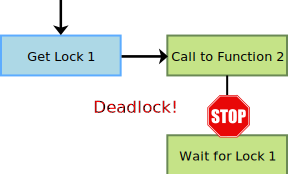
\includegraphics[height=0.3\textheight]{slides/kernel-driver-development-concurrency/deadlock-same-lock.pdf}
    \end{center}
  \item Holding multiple locks is risky!
    \begin{center}
      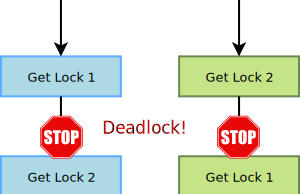
\includegraphics[height=0.3\textheight]{slides/kernel-driver-development-concurrency/deadlock-two-locks.pdf}
    \end{center}
  \end{itemize}
\end{frame}

\begin{frame}
  \frametitle{Kernel lock validator}
  \begin{itemize}
  \item From Ingo Molnar and Arjan van de Ven
    \begin{itemize}
    \item Adds instrumentation to kernel locking code
    \item Detect violations of locking rules during system life, such
      as:
      \begin{itemize}
      \item Locks acquired in different order (keeps track of locking
        sequences and compares them).
      \item Spinlocks acquired in interrupt handlers and also in
        process context when interrupts are enabled.
      \end{itemize}
    \item Not suitable for production systems but acceptable overhead
      in development.
    \end{itemize}
  \item See \kerneldoc{lockdep-design.txt} for details
  \end{itemize}
\end{frame}

\begin{frame}
  \frametitle{Alternatives to Locking}
  \begin{itemize}
  \item As we have just seen, locking can have a strong negative
    impact on system performance. In some situations, you could do
    without it.
    \begin{itemize}
    \item By using lock-free algorithms like \emph{Read Copy Update}
      (RCU).
    \item RCU API available in the kernel (See
      \url{http://en.wikipedia.org/wiki/RCU}).
    \item When available, use atomic operations.
    \end{itemize}
  \end{itemize}
\end{frame}

\begin{frame}[fragile]
  \frametitle{Atomic Variables 1/2}
  \begin{itemize}
  \item Useful when the shared resource is an integer value
  \item Even an instruction like \code{n++} is not guaranteed to be
    atomic on all processors!
  \item Atomic operations definitions
    \begin{itemize}
    \item \mint{c}+#include <asm/atomic.h>+
    \end{itemize}
  \item \code{atomic_t}
    \begin{itemize}
    \item Contains a signed integer (at least 24 bits)
    \end{itemize}
  \item Atomic operations (main ones)
    \begin{itemize}
    \item Set or read the counter:
      \begin{itemize}
      \item \mint{c}+void atomic_set(atomic_t *v, int i);+
      \item \mint{c}+int atomic_read(atomic_t *v);+
      \end{itemize}
    \item Operations without return value:
      \begin{itemize}
      \item \mint{c}+void atomic_inc(atomic_t *v);+
      \item \mint{c}+void atomic_dec(atomic_t *v);+
      \item \mint{c}+void atomic_add(int i, atomic_t *v);+
      \item \mint{c}+void atomic_sub(int i, atomic_t *v);+
      \end{itemize}
    \end{itemize}
  \end{itemize}
\end{frame}

\begin{frame}[fragile]
  \frametitle{Atomic Variables 2/2}
  \begin{itemize}
  \item Similar functions testing the result:
    \begin{itemize}
    \item \mint{c}+int atomic_inc_and_test(...);+
    \item \mint{c}+int atomic_dec_and_test(...);+
    \item \mint{c}+int atomic_sub_and_test(...);+
    \end{itemize}
  \item Functions returning the new value:
    \begin{itemize}
    \item \mint{c}+int atomic_inc_return(...);+
    \item \mint{c}+int atomic_dec_return(...);+
    \item \mint{c}+int atomic_add_return(...);+
    \item \mint{c}+int atomic_sub_return(...);+
    \end{itemize}
  \end{itemize}
\end{frame}

\begin{frame}[fragile]
  \frametitle{Atomic Bit Operations}
  \begin{itemize}
  \item Supply very fast, atomic operations
  \item On most platforms, apply to an unsigned long type.
  \item Apply to a void type on a few others.
  \item Set, clear, toggle a given bit:
    \begin{itemize}
    \item \mint{c}+void set_bit(int nr, unsigned long * addr);+
    \item \mint{c}+void clear_bit(int nr, unsigned long * addr);+
    \item \mint{c}+void change_bit(int nr, unsigned long * addr);+
    \end{itemize}
  \item Test bit value:
    \begin{itemize}
    \item \mint{c}+int test_bit(int nr, unsigned long *addr);+
    \end{itemize}
  \item Test and modify (return the previous value):
    \begin{itemize}
    \item \mint{c}+int test_and_set_bit(...);+
    \item \mint{c}+int test_and_clear_bit(...);+
    \item \mint{c}+int test_and_change_bit(...);+
    \end{itemize}
  \end{itemize}
\end{frame}
